\chapter{Network Analysis}
\section{Network analysis}
\subsection{Electrical networks}
Note that the system interconnects in a complex pattern allowing for multiple current paths. How to determine voltage and current flows?
\begin{figure}[H]
	\centering
	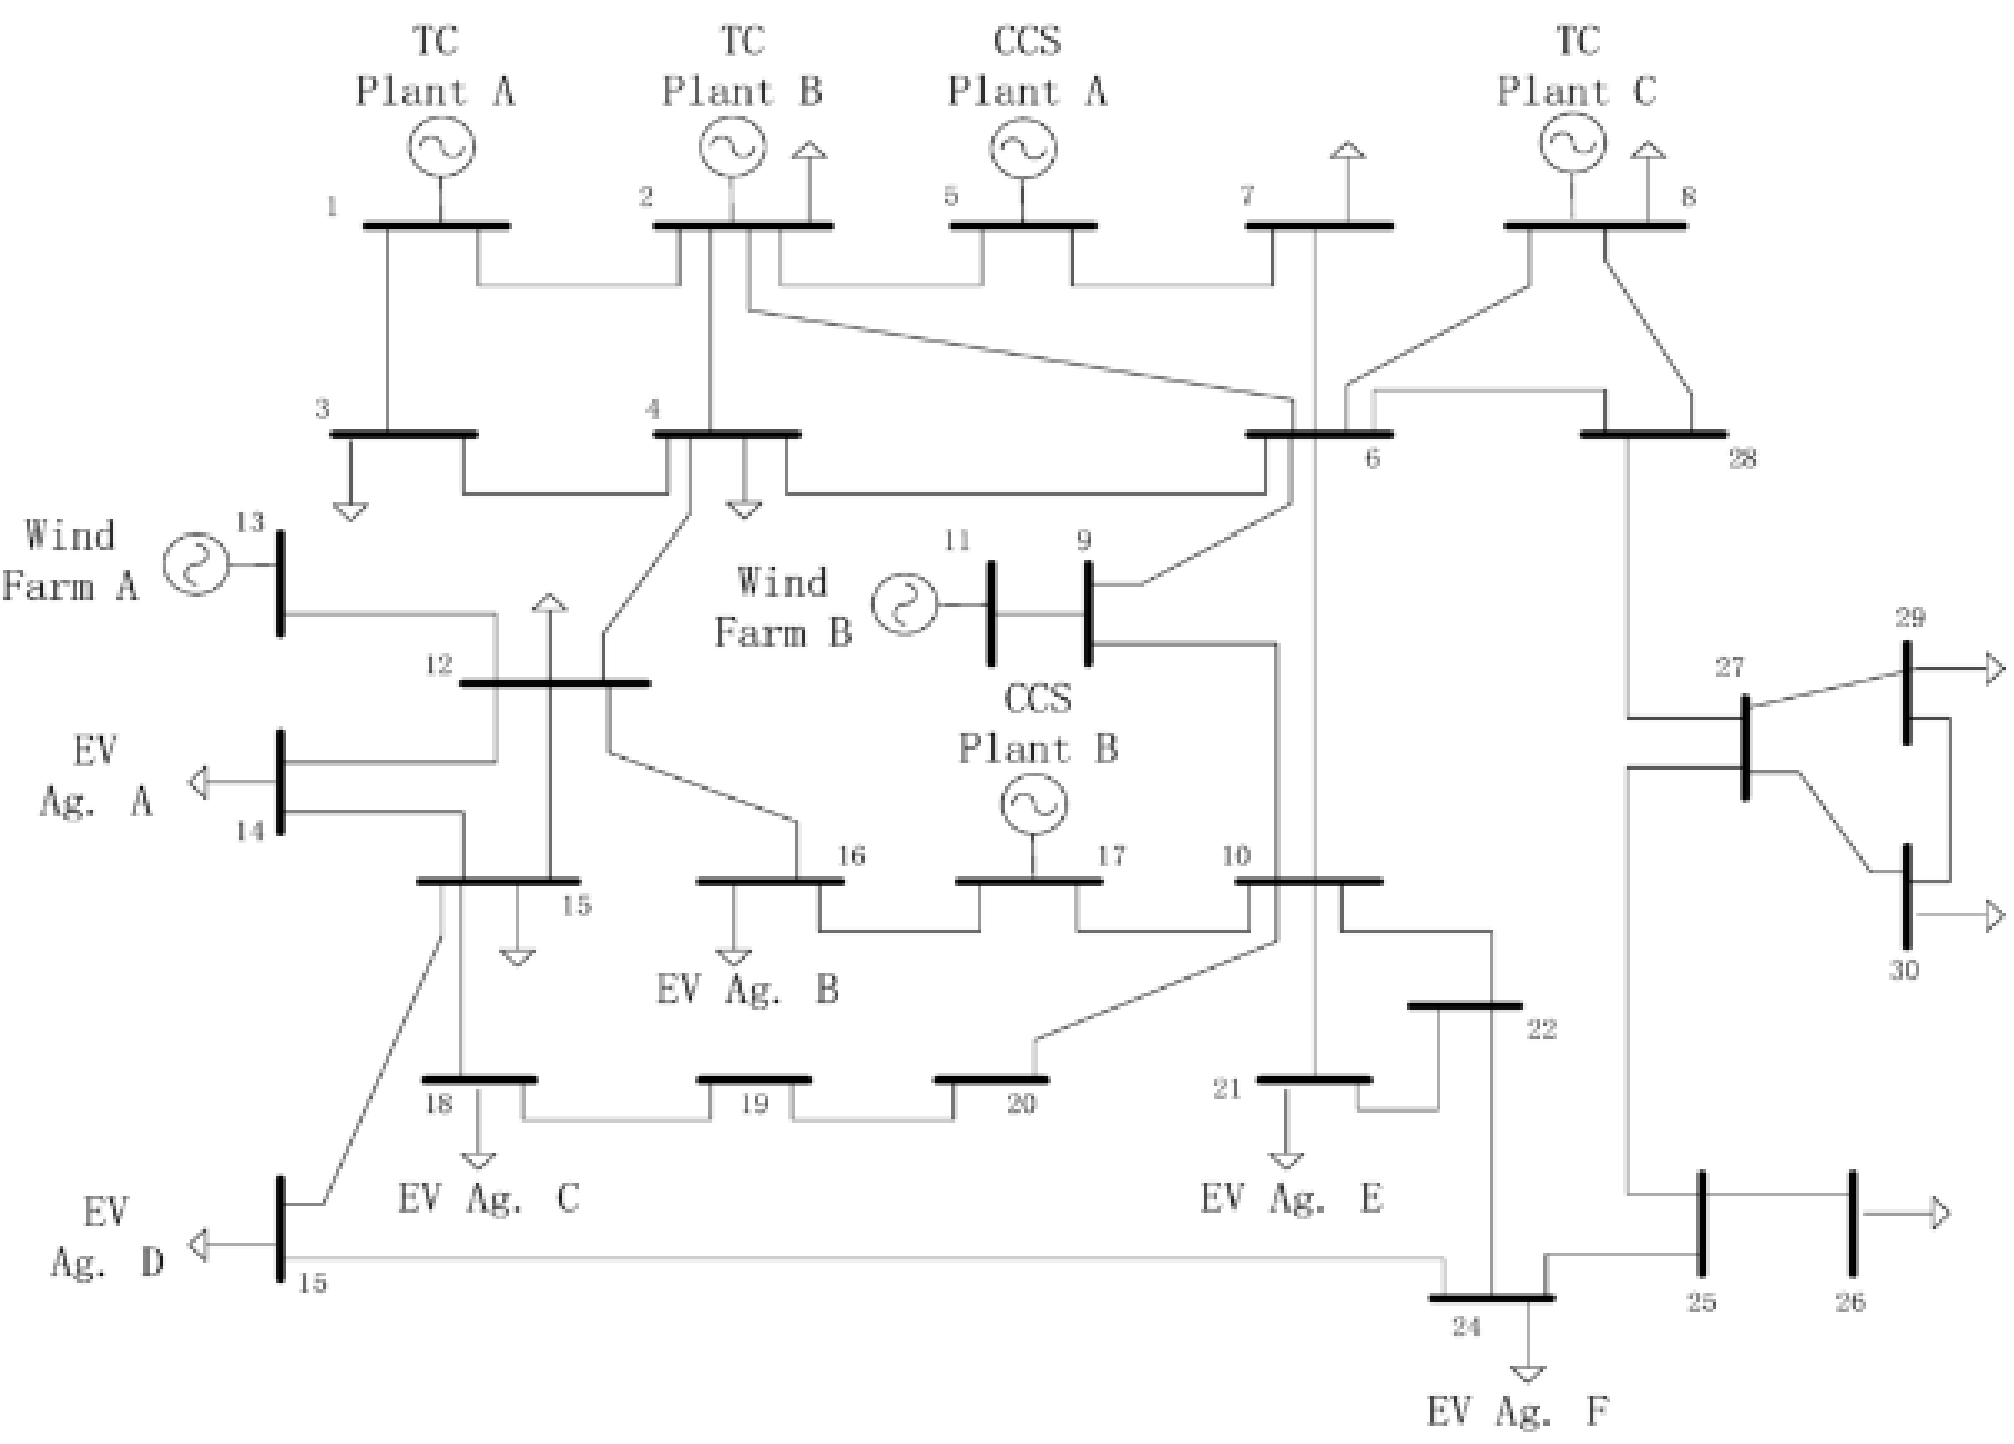
\includegraphics[width = \textwidth]{./img/figure45.png}
	\caption{Network at a works.}
\end{figure}
\subsection{Split distribution system - high integrity}
Non-essential loads (NE) are divided equally between two generators. Essential loads (E) have a cross-over connection capability either manual or automatic. This system ensures the integrity of the electrical system in case of generator failure.
\begin{figure}[H]
	\centering
	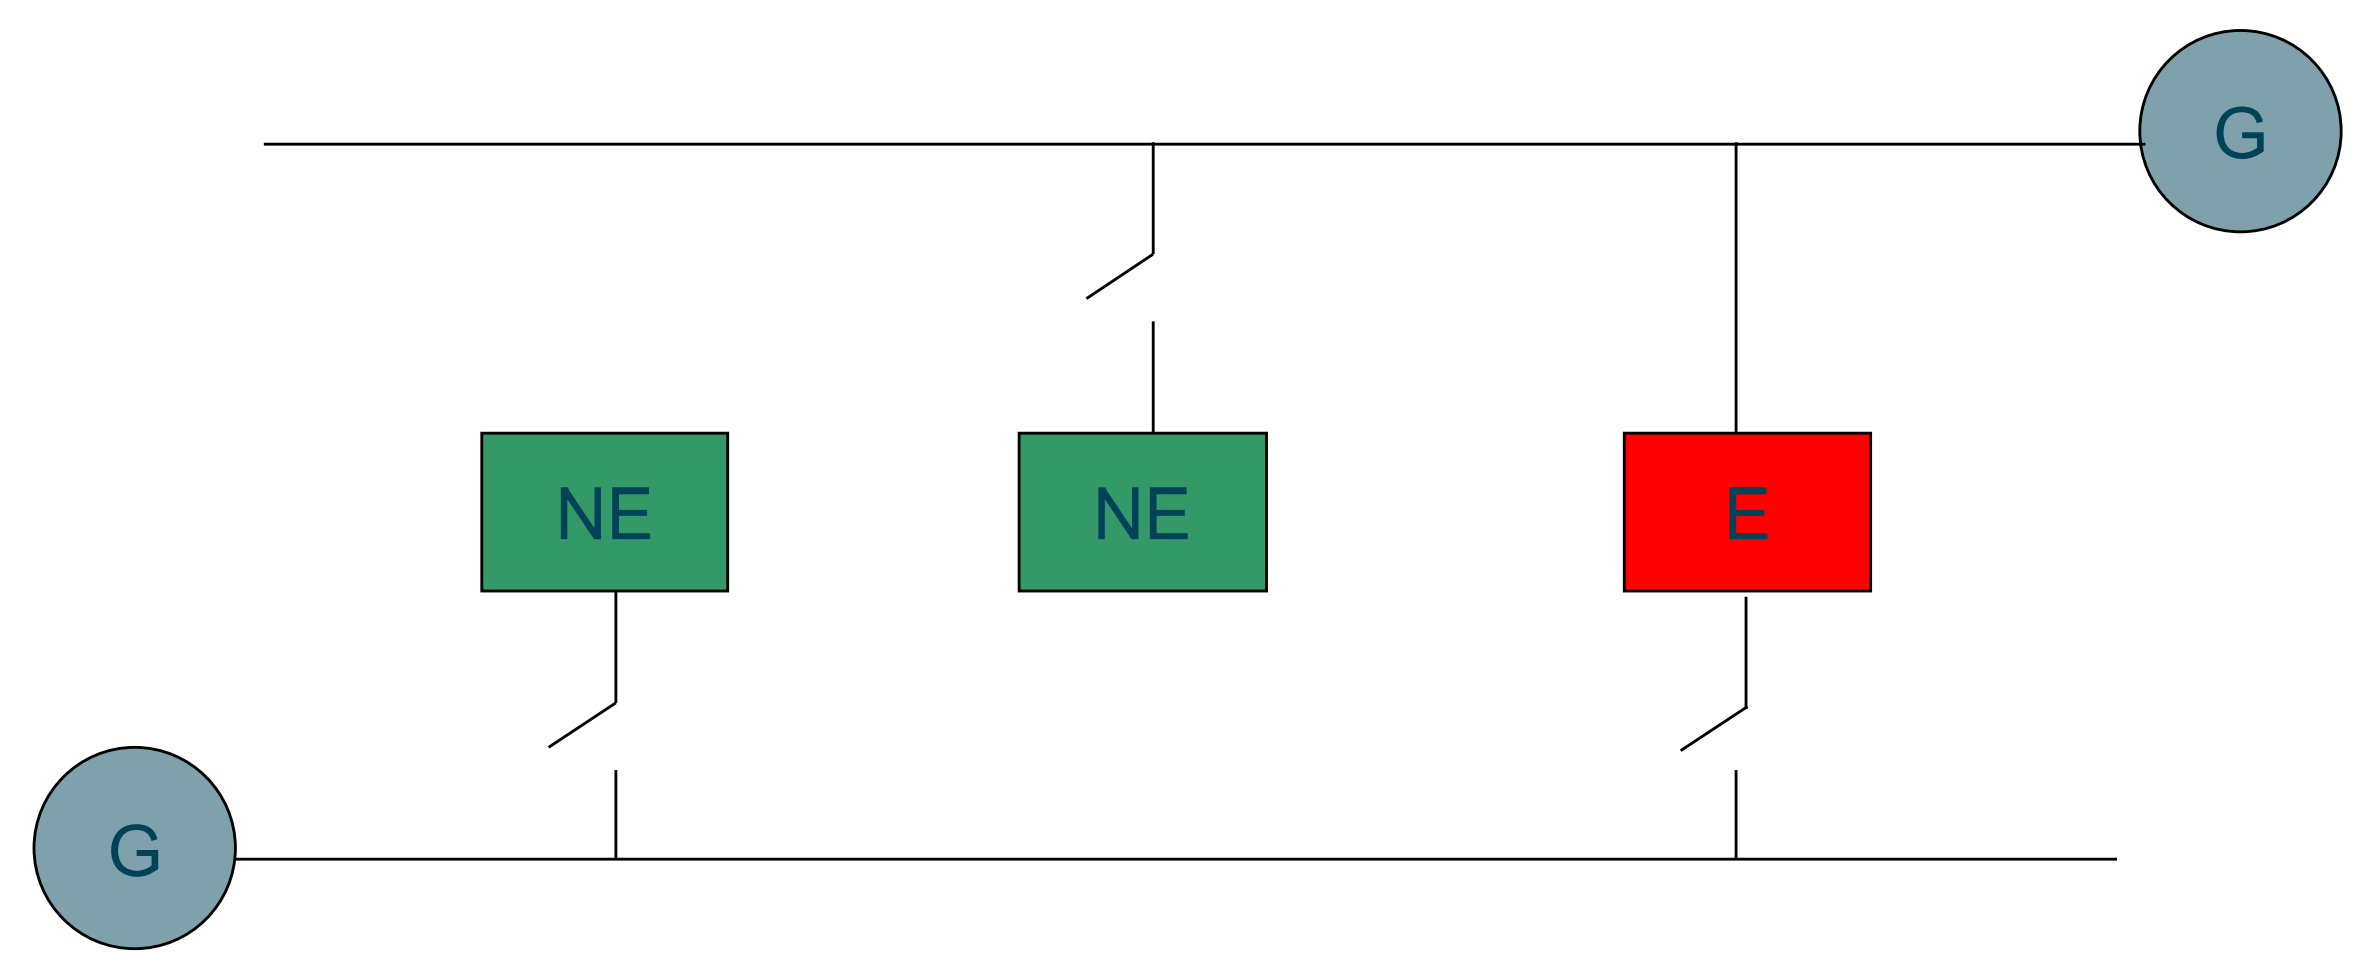
\includegraphics[width = \textwidth]{./img/figure46.png}
	\caption{Split distribution system - high integrity.}
\end{figure}
\subsection{Tree distribution}
Electrical power is generated (generators can be used in parallel) by the main generators to supply loads distibuted around the vessel. A small emergency generator is used as back-up to supply the emergency switchboard, which is usually supplied by the main board. 
\begin{figure}[H]
	\centering
	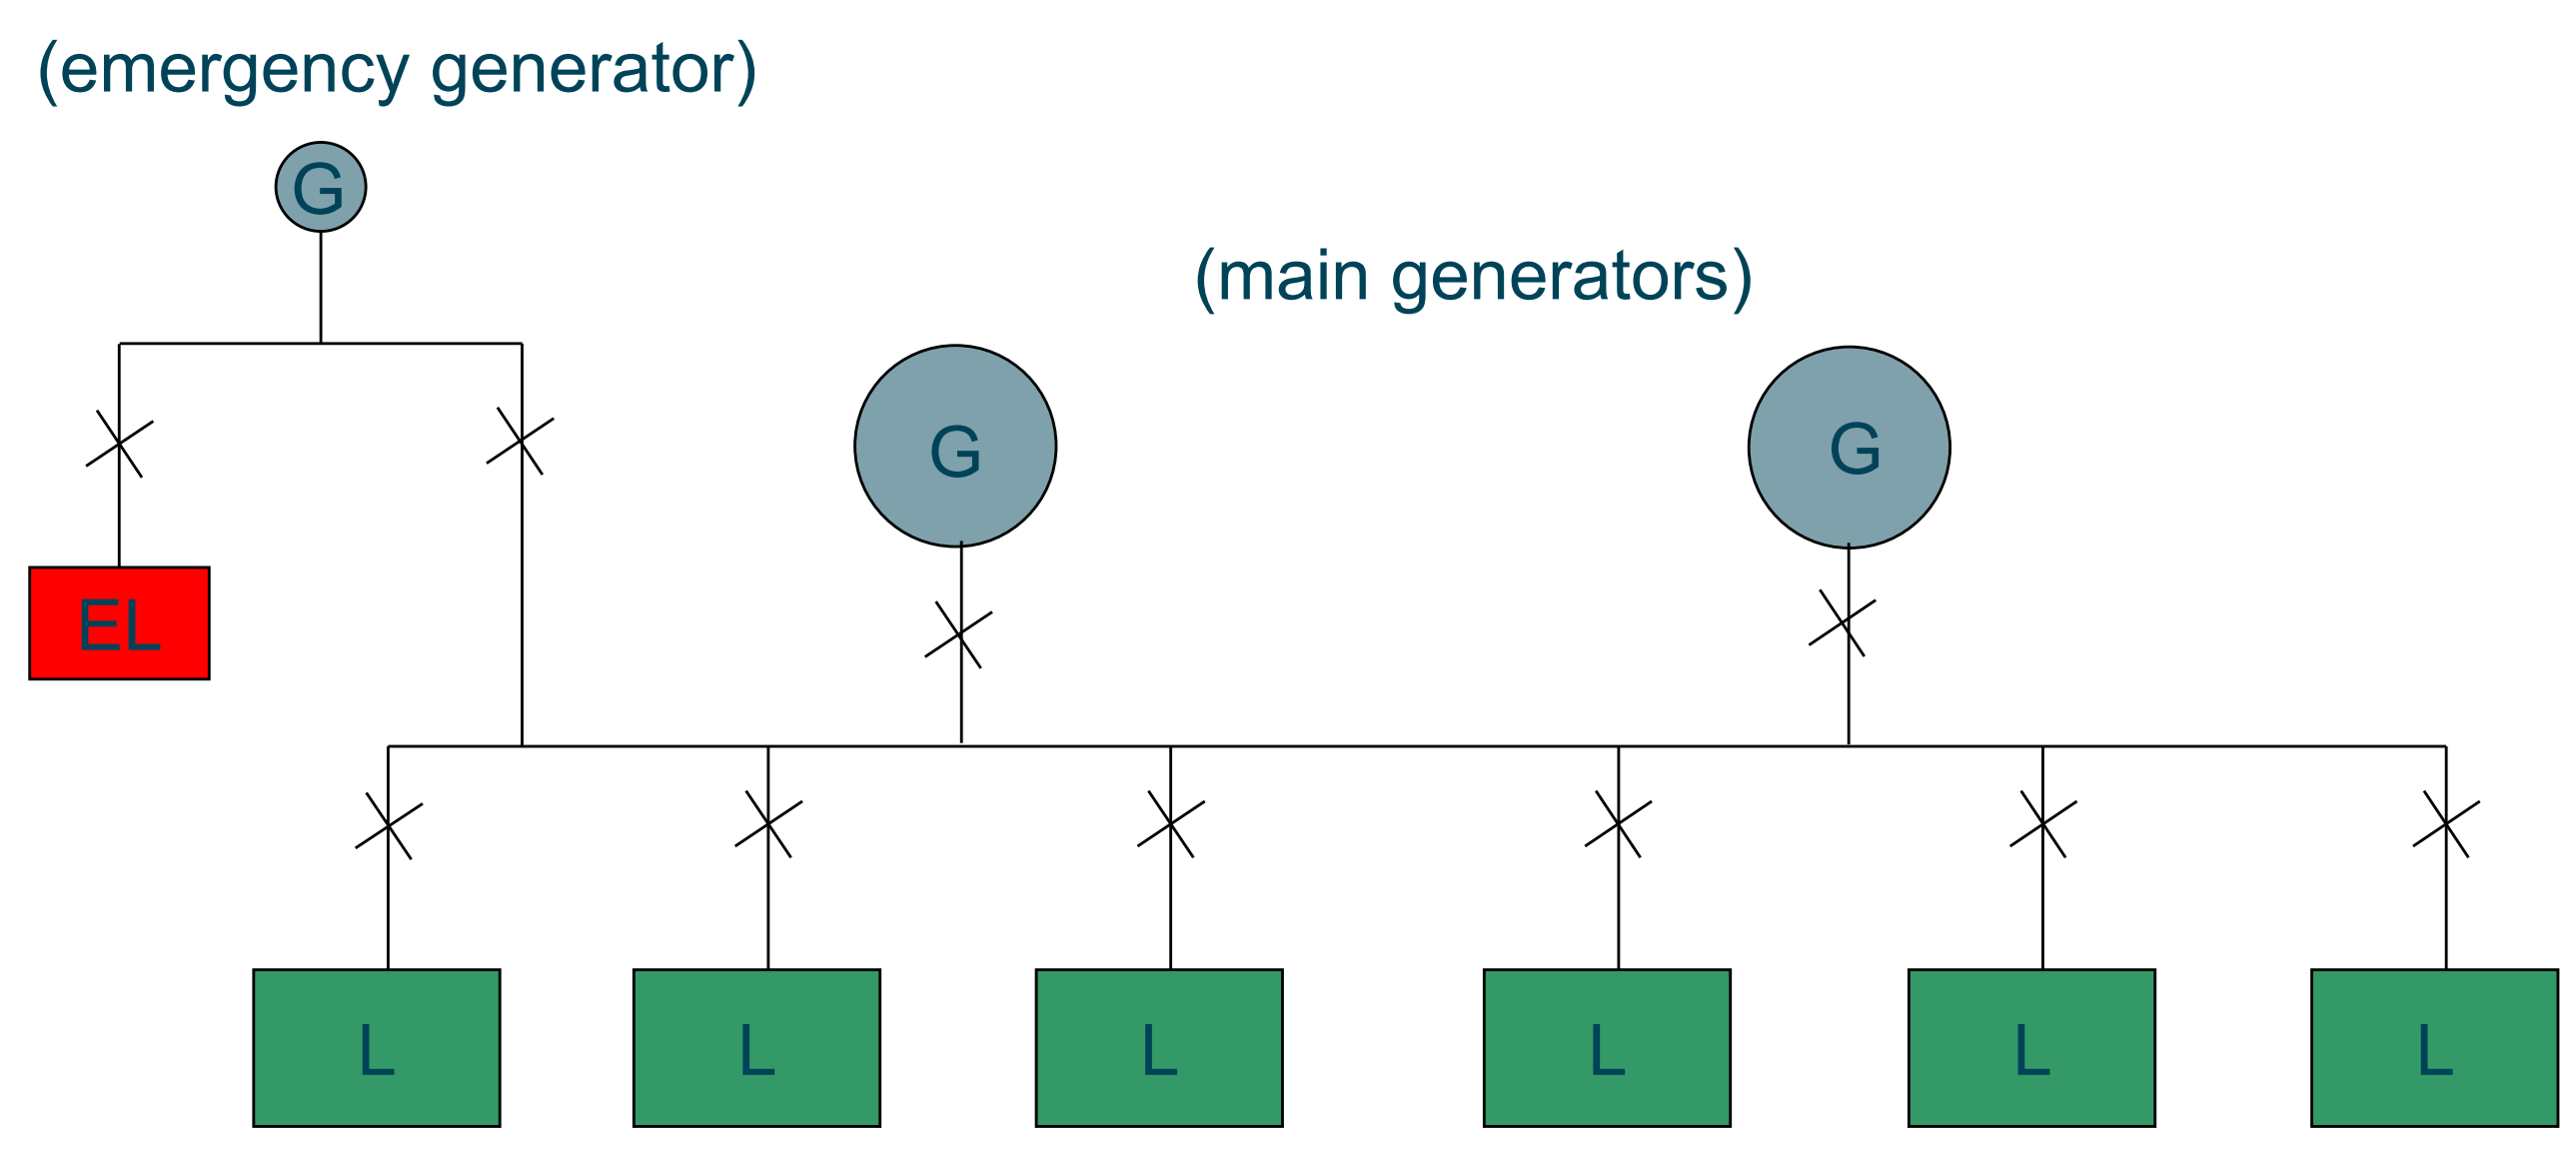
\includegraphics[width = \textwidth]{./img/figure47.png}
	\caption{Tree distribution.}
\end{figure}
\subsection{Ring networks - grids}
\begin{figure}[H]
	\centering
	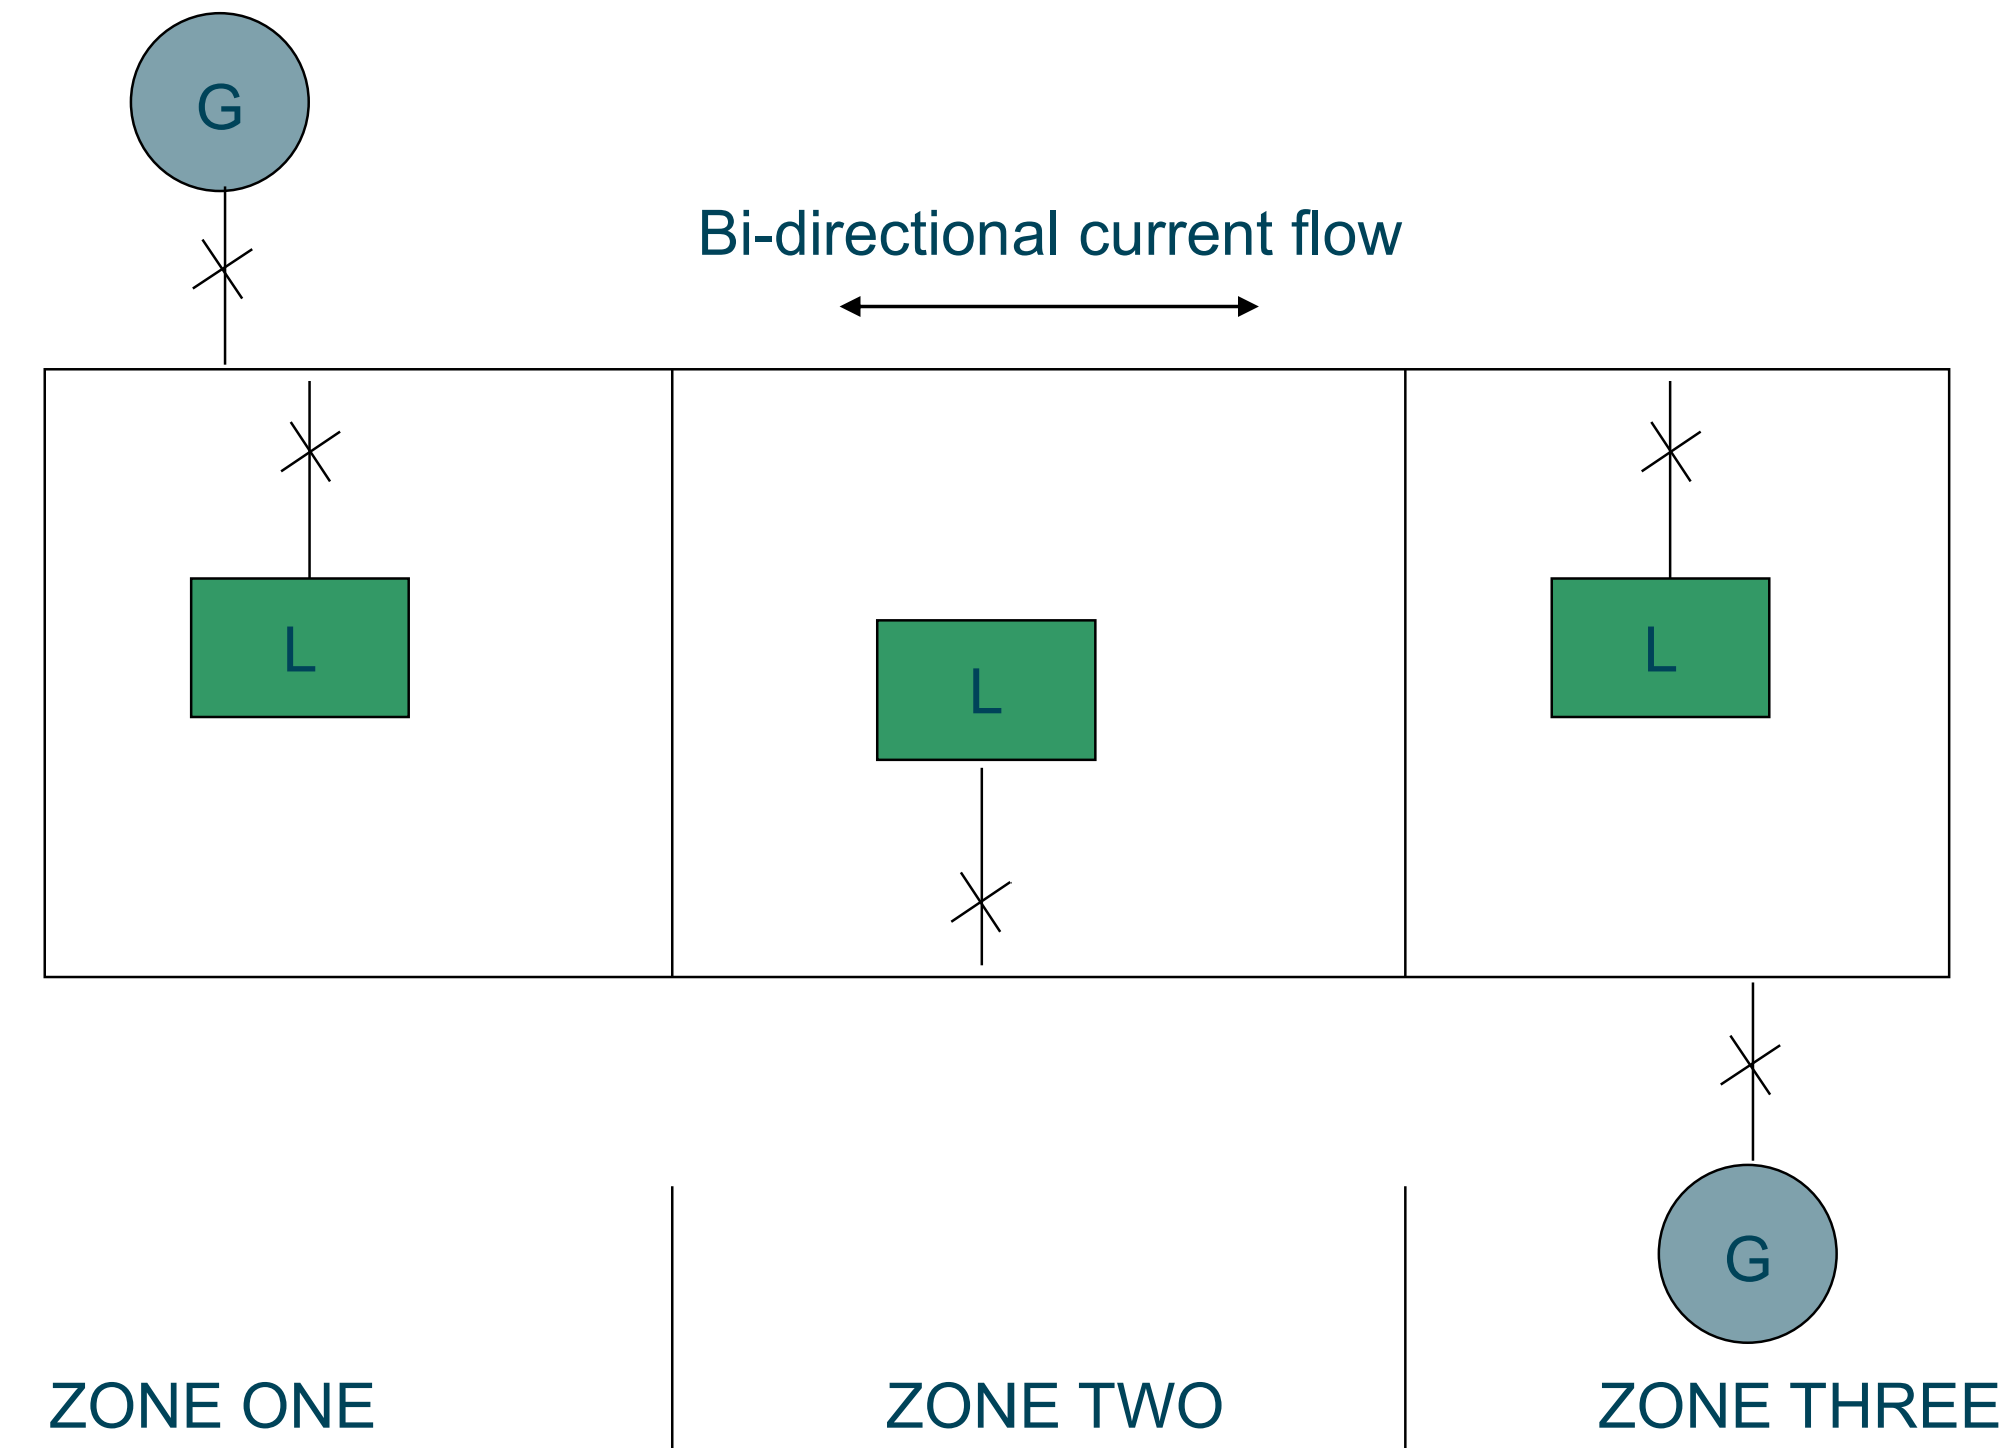
\includegraphics[width = \textwidth]{./img/figure48.png}
	\caption{Ring networks - grids.}
\end{figure}
\subsection{Network analysis}
It is essential to be able to analyse the performance of power systems whatever their design both during normal operating conditions and under fault (short-circuit) conditions. The analysis in normal steady-state operation is called a \textbf{power-flow study (load-flow study)} and it involves determing the voltages, current and real and reactive power flows in system under given load conditions. Earlier in the course, we examined the impact of an induction motor start. However, that was a single network and relatively straight forward. For more complex system, matrix methods are best used.

Today most power-flow studies are done by computer. The purpose of power flow studies is to plan ahead to be able to account for various hypothetical situations and understand steady-state, transient and faulted conditions. For instance, what if a transmission line within the power system properly supplying loads must be taken offline for maintenance. Can the remaining lines in the system handle the required loads without exceeding their rated parameters? For instance, what happens if a switchboard in a ship becomes faulty and need to be isolated or what happens when new equipment is fitted to an existing network?
\subsection{Techniques for power-flow studies}
A power-flow study (load-flow study) is an analysis of the voltages, currents and power flows in a power system and we will consider steady-state conditions. In such a study, we make an assumption:
\begin{enumerate}
	\item Either a \textbf{voltage} at a bus or the \textbf{power} being supplied to a bus for each bus in the power system
	\item We then determine the magnitude and phase angles of the bus voltages, line currents, etc. that would result from the assumed combination of voltages and power flows
	\item We use iterative methods of analysis to resolve
\end{enumerate}
\subsection{Power flow calculations}
The simplest way to perform power-flow calculations is by iteration. 
\begin{enumerate}
	\item Create a bus admittance matrix $Y_{bus}$ for the power system.
	\begin{itemize}
		\item \begin{gather}
			Y = \frac{1}{Z} = \left(G + jB\right)
		\end{gather}
		$G$ is conductance, $B$ is called susceptance and may be positive or negative. Note that: 
		\begin{gather}
			G = \frac{1}{R}, \quad B \neq \frac{1}{X}
		\end{gather}
	\end{itemize}
	\item Make an initial estimate for the voltages at each bus in the system (ideally something that is reasonable)
	\item Update the voltage estimate for each bus (one at a time), based on the estimates for the voltages and power flows at every other bus and the values of the bus admittance matrix (the voltage at a given bus depends on the voltages at all of the other buses in the system so even the updated voltage will not be correct but it will usually be closer to the answer than the original estimate). - An iterative method
	\item Repeat this process to make the voltages at each bus approaching the correct answers closer and closer\dots
\end{enumerate}
There are three types of defined bus:
\begin{itemize}
	\item Load bus
	\item Generator bus
	\item Slack bus
\end{itemize}
The process involves defining these buses and then sticking with that definition.
\subsection{Basic techniques for power-flow studies}
The equations used to update the estimates differ for different types of buses. Each bus in a power system can be classified to one of three types.
\begin{enumerate}
	\item \textbf{\underline{Load bus}} (PQ bus) - a bus at which the real and reactive power are specified, and for which the bus voltage will be calculated. \textbf{Real and reactive powers supplied to a power system are defined to be positive}, while the \textbf{powers consumed from the system are defined to be negative. All busses having no generators are load busses}
	\item \textbf{\underline{Generator bus}} (PV bus) - a bus at which the magnitude of the voltage is kept constant by adjusting the field current of a synchronous generator on the bus (\textbf{remember} - increasing the field current of the generator increases both the reactive power supplied by the generator and the terminal voltage of the system). We assume that the field current is adjusted to maintain a constant voltage $V_T$. We also know that increasing the prime mover's governor set points increases the power that the generator supplies to the power system and the frequency. Therefore, we can \textit{specify} the magnitude of the bus voltage and real power supplied
	\item \textbf{\underline{Slack bus}} (swing bus) - a \underline{special generator bus} serving as the reference bus for the power system. Its voltage is assumed to be fixed in both magnitude and phase (for instance, $1\angle\SI{0}{\degree}\, \si{pu}$). The real and reactive powers are uncontrolled: the bus supplies whatever real or reactive power is necessary to make the power flows in the system balance. 
\end{enumerate}
\subsection{Approach to analysis}
The most common approach to power-flow analysis is based on the bus admittance matrix $Y_{bus}$. However, this matrix is slightly different from the system previously since the internal impedances of generators and loads connected to the system are not included in the $Y_{bus}$. Instead, they are accounted for as specified real and reactive powers input and output from the buses.
\begin{figure}[H]
	\centering
	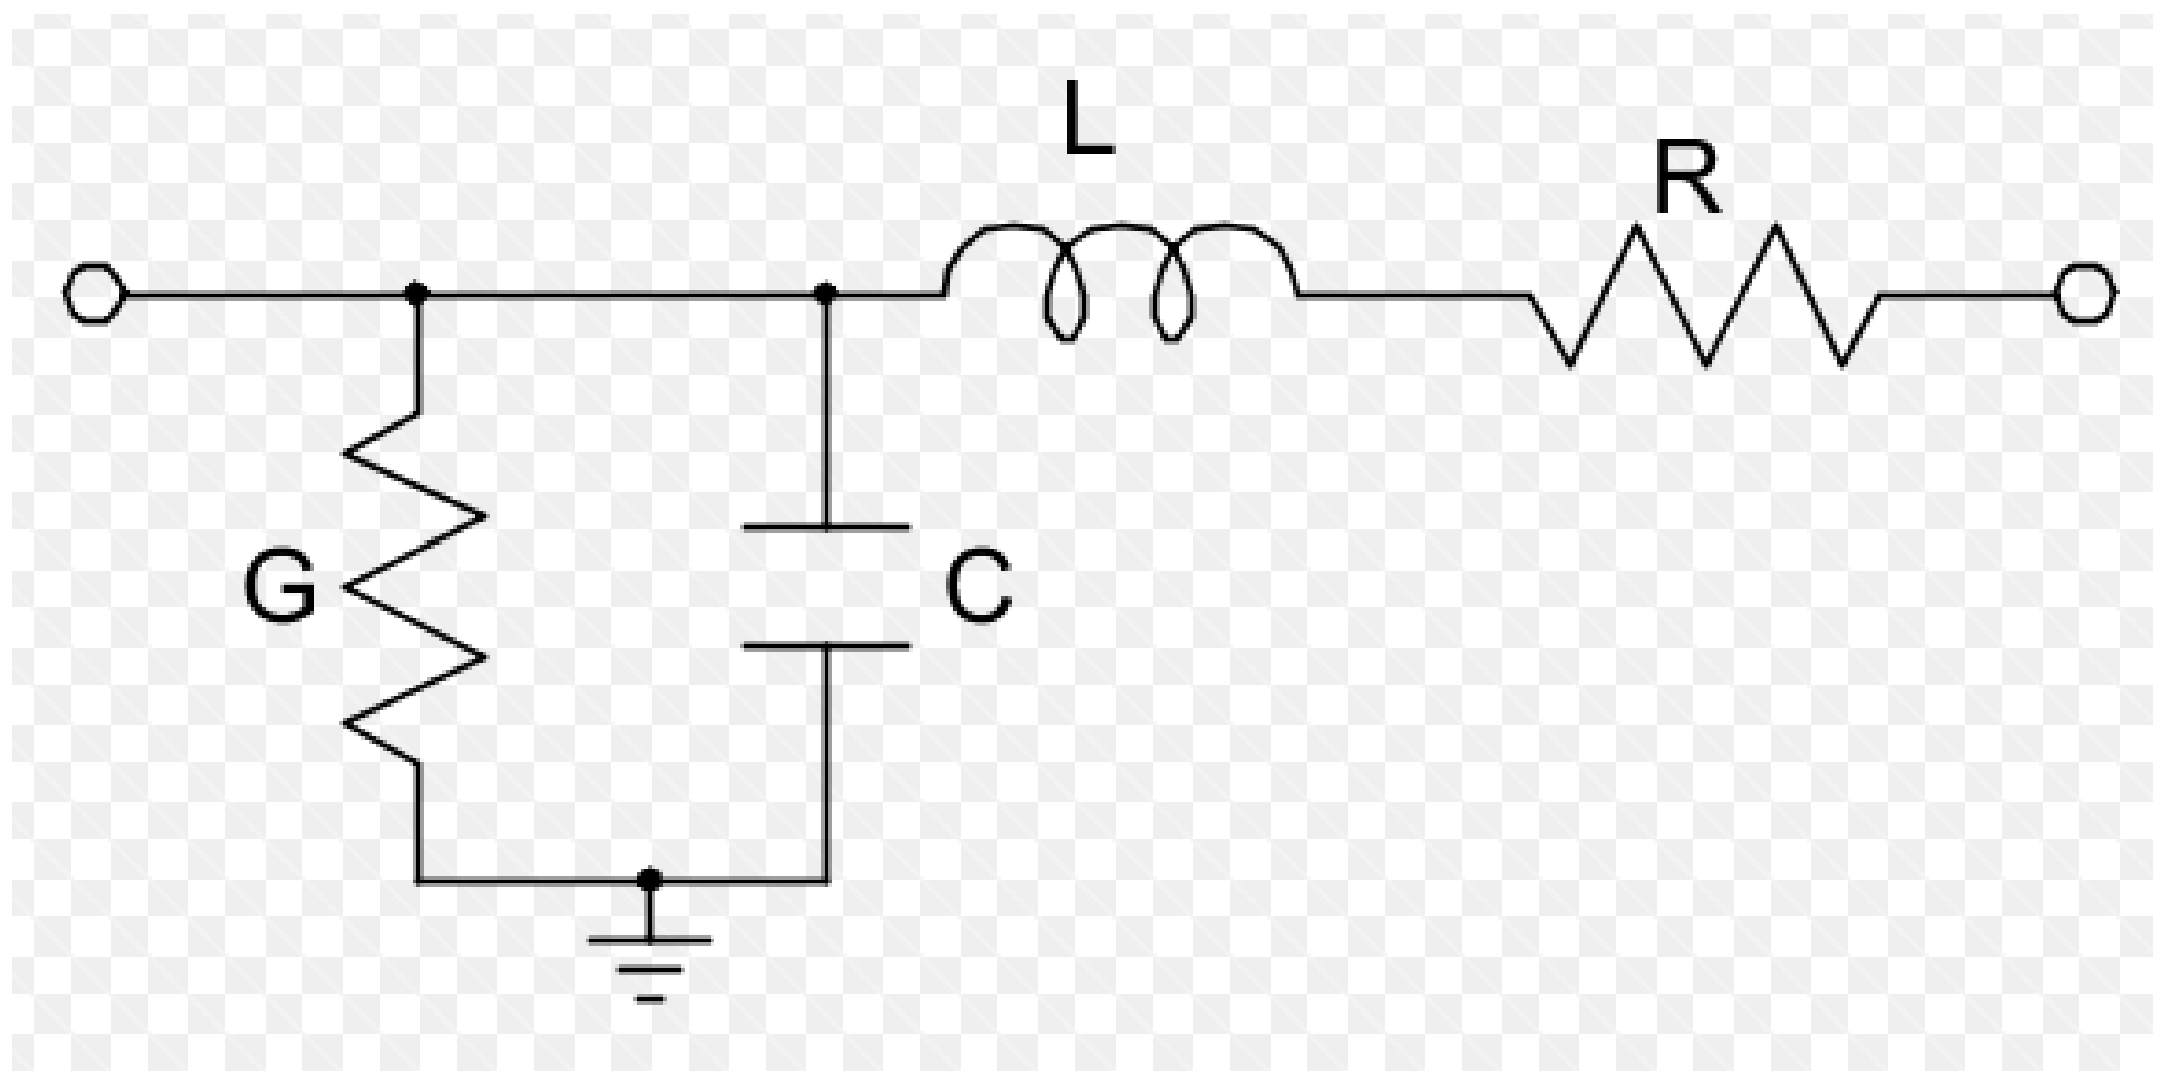
\includegraphics[width = 0.5\textwidth]{./img/figure49.png}
	\caption{Transmission line: only L and R are used in the $Y_{bus}$.}
\end{figure}
\subsection{Constructing $Y_{bus}$ for power-flow analysis}
Example 1: A simple power system has 4 busses, 5 transmission lines, 1 generator and 3 loads.
\begin{table}[H]
	\centering
	\begin{tabular}{@{}lll@{}}
		\toprule
		\textbf{line no.} & \textbf{Bus to bus} & \textbf{Series $Y$ (pu)}\\
		\midrule
		1 & 1-2 & $0.5882 - j2.3529$\\
		2 & 2-3 & $0.3846 - j1.9231$\\
		3 & 2-4 & $0.5882 - j2.3529$\\
		4 & 3-4 & $1.1765 - j4.7059$\\
		5 & 4-1 & $1.1765 - j4.7059$\\
		\bottomrule
	\end{tabular}
	\caption{Example 1 series per unit admittances.}
\end{table}
\begin{table}[H]
	\centering
	\begin{tabular}{@{}ll@{}}
		\toprule
		\multicolumn{2}{l}{\textbf{Table of busses}}\\
		\midrule
		Bus 1 & Slack bus\\
		Bus 2 & Load bus\\
		Bus 2 & Load bus\\		
		Bus 2 & Load bus\\
		\bottomrule
	\end{tabular}
	\caption{Example 1 table of busses.}
\end{table}
\begin{figure}[H]
	\centering
	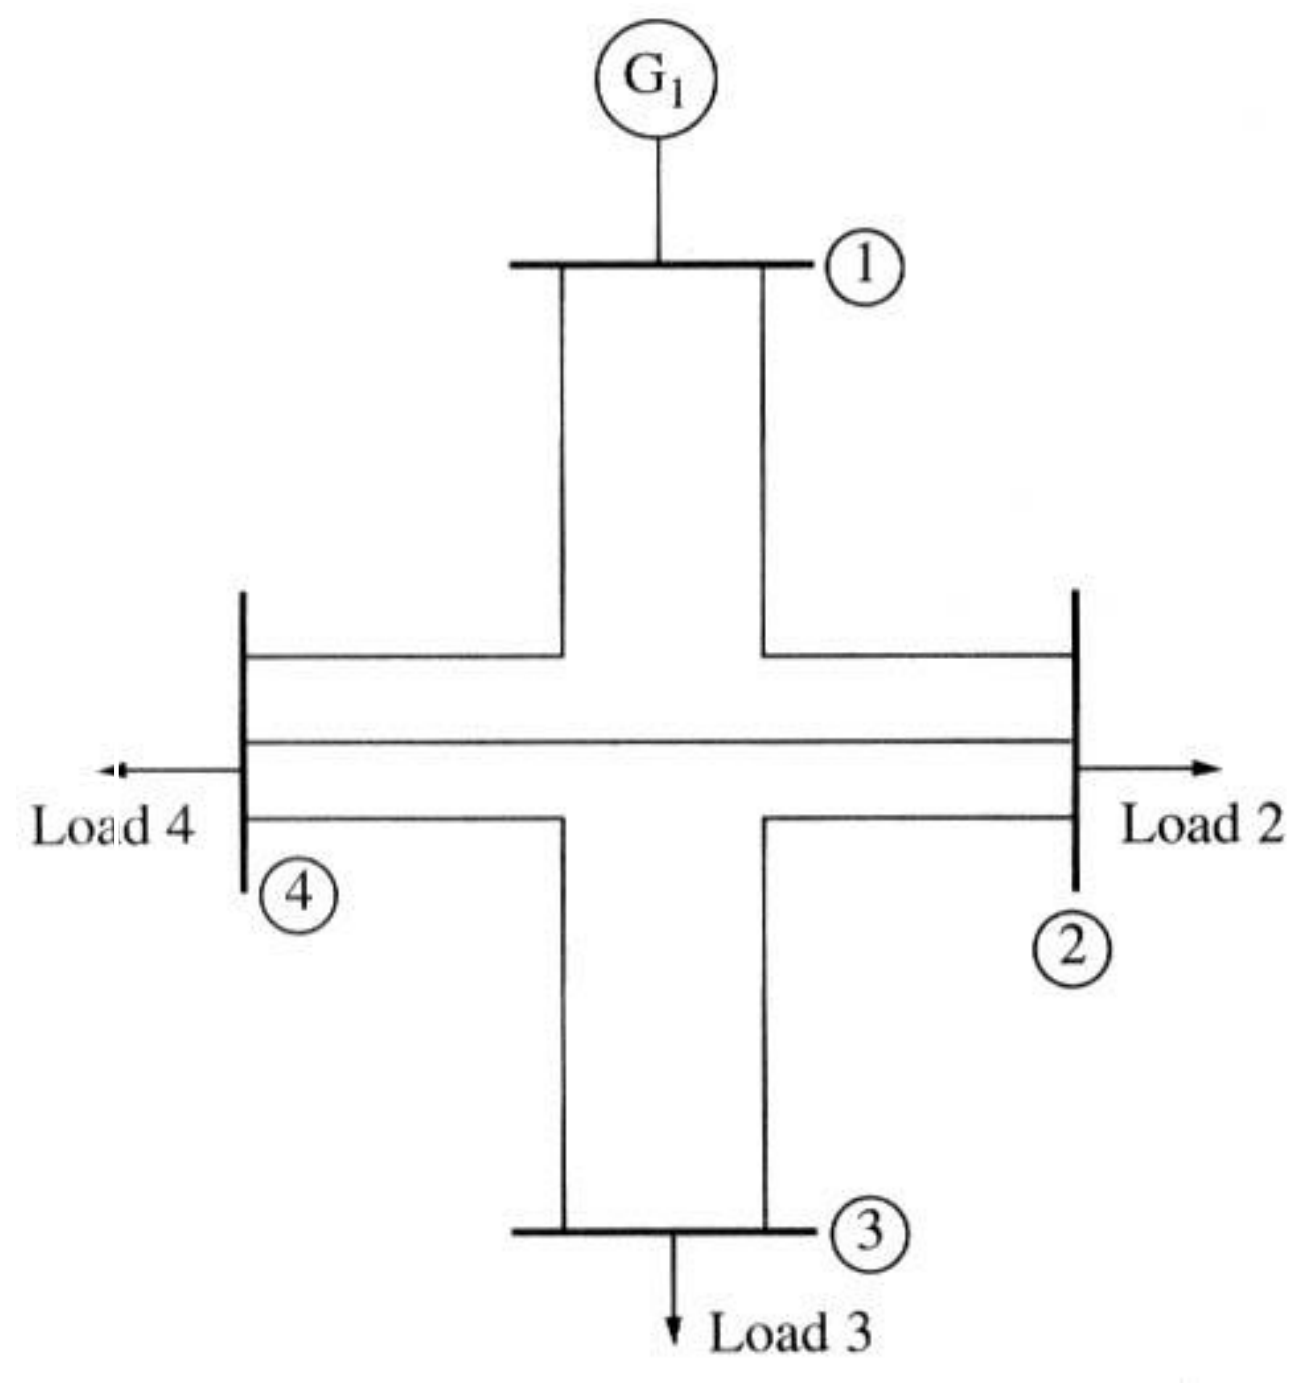
\includegraphics[width = 0.7\textwidth]{./img/figure50.png}
	\caption{Transmission line: only L and R are used in the $Y_{bus}$.}
\end{figure}
The shunt admittances of the transmission lines are ignored. In this case, the $Y_{ii}$ terms of the bus admittance matrix can be constructed by summing the admittances of all transmission lines connected to each bus, and the $Y_{ij}\, (i \neq j)$ terms are just the negative of the line admittances stretching between busses $i$ and $j$. Therefore, for instance, the term $Y_{11}$ will be the sum of the admittances of all transmission lines connected to bus 1. which are the lines 1 and 5, so:
\begin{gather}
	Y_{11} = 1.7647 - j7.0588\, \si{pu}
\end{gather}
Note: if the shunt admittances of the transmission lines are not ignored, the self admittance $Y_{ii}$ at each bus would also include half of the shunt admittance of each transmission line connected to the bus.

The term $Y_{12}$ is defined as the negative of all the admittances stretching between bus 1 and bus 2, which will be the negative of the admittance of the transmission line 1, so:
\begin{gather}
	Y_{12} = -0.5882 + j2.3529
\end{gather}
The complete bus admittance matrix can be obtained by repeating these calculations for every term in the matrix.
\begin{gather}
	Y_{bus} = \begin{bmatrix}
		1.7647-j7.0588 & -0.5882 + j2.3529 & 0 & -1.1765 + j4.7059\\
		-0.5882 + j2.3529 & 1.5611-j6.5290 & -0.3746 + j1.9231 & -0.5882 + j2.3529\\
		0 & -0.3846+j1.9231 & 1.5611-j6.6290 & -1.1765 + j4.7059\\
		-1.1765+j4.7059 & -0.5882 + j2.3529 & -1.1765 + j4.7059 & 2.9412 - j11.7647
		\end{bmatrix}
\end{gather}
\subsection{Power-flow analysis equations}
The basic equation for power-flow analysis is derived fron the nodal analysis equations for the power system: 
\begin{gather}
	Y_{bus}V = I
\end{gather}
For the four-bus power system shown above, becomes:
\begin{gather}
	\begin{bmatrix}
		Y_{11} & Y_{12} & Y_{13} & Y_{14}\\
		Y_{21} & Y_{22} & Y_{23} & Y_{24}\\
		Y_{31} & Y_{32} & Y_{33} & Y_{34}\\
		Y_{41} & Y_{42} & Y_{43} & Y_{44}
	\end{bmatrix} \begin{bmatrix}
		V_1\\
		V_2\\
		V_3\\
		V_4
	\end{bmatrix}=\begin{bmatrix}
		I_1\\
		I_2\\
		I_3\\
		I_4
	\end{bmatrix}
\end{gather}
where $Y_{ij}$ are the elements of the bus admittance matrix, $V_i$ are the bus voltages, and $I_i$ are the currents injected at each node. FOr bus 2 in this system, this equation reduces to:
\begin{gather}
	Y_{21}V_1 + Y_{22}V_2 + Y_{23}V_3 + Y_{24}V_4 = I_2
\end{gather}
However, real loads are specified in terms of real and reactive powers, not as currents. The relationship between per-unit real and reactive power supplied to the system at a bus and the per-unit current injected into the system at that bus is:
\begin{gather}
	S = VI^* = P+jQ
\end{gather}
where $V$ is the per-unit voltage at the bus, $I^*$ is the complex conjugate of the per-unit current injected at the bus, $P$ and $Q$ are per-unit real and reactive powers. Therefore, for instance, the current injected at bus 2 can be found as:
\begin{gather}
	V_2 I^*_2 = P_2 + jQ_2 \rightarrow I^*_2 = \frac{P_2 + jQ_2}{V_2}
\end{gather}
Now the next steps are
\begin{enumerate}
	\item To switch $I^*_2$ and $V_2$ to use $I_2$ and $v_2^*$
	\item In doing so we have to change to $P$-$Q$ to keep sense
	\item Substitute $I$ for the relationships for $I = YZ$
\end{enumerate}
Implementing for $V_2$, yields\dots
\begin{gather}
	V_2 = \frac{1}{Y_{22}}\left[\frac{P_2-jQ_2}{V_2^*}-\left(Y_{21}V_1+Y_{23}V_3+Y_{24}V_4\right)\right]
\end{gather}
Similar equations can be created for each load bus in the power system.
\subsubsection{Gauss-Siedel iterative method}
Basic procedure:
\begin{enumerate}
	\item Calculate the bus admittance matrix $Y_{bus}$ including the admittances of all transmission lines, transformers, etc., between busses but exclides the admittances of the loads or generators themselves.
	\item Select a slack bus: one of the busses in the power system, whose voltage will arbitrarily be assumed as $1.0\angle\SI{0}{\degree}$.
	\item Select initial estimates for all bus voltages: usually, the voltage at every load bus is assumed as $1.0\angle\SI{0}{\degree}$ (flat start) lead to good covergence. Write voltage equations for every other bus in the system. The generic form is:
	\begin{gather}
		V_i = \frac{1}{Y_{ii}}\left(\frac{P_i-jQ_i}{V_i^*}-\sum^N_{k=1,\,k\neq i}T_{ik}V_k\right)
	\end{gather}
	\item Calculate an updated estimate of the voltage at each load bus in succession (except for the slack bus).
	\item Compare the differences between the old and new voltage estimates: if the differences are less than some specified tolerance for all busses, stop. Otherwise, repeat step 5.
	\item Confirm that the resulting solution is reasonable.
\end{enumerate}
\subsection{Example 2}
In a 2-bus power system, a generator attached to bus 1 and loads attached to bus 2. The series impedance of a single transmission line connecting them is $0.1 +j0.5\, \si{pu}$. The shunt admittance of the line may be negelected. Assume that bus 1 is the slack bus and that it has a voltage $V_1 = 1.0\angle\SI{0}{\degree}\,\si{pu}$. Real and reactive powers \underline{supplied} to the loads from the system at bus 2 are $P_2 = \SI{-0.3}{pu}$, $Q_2 = \SI{0.2}{pu}$. Determine voltages at each bus for the specified load conditions.
\begin{table}[H]
	\centering
	\begin{tabular}{@{}ll@{}}
		\toprule
		\multicolumn{2}{l}{\textbf{Table of busses}}\\
		\midrule
		Bus 1 & Slack bus\\
		Bus 2 & Load bus\\
		\bottomrule
	\end{tabular}
	\caption{Example 2 table of busses.}
\end{table}
\begin{figure}[H]
	\centering
	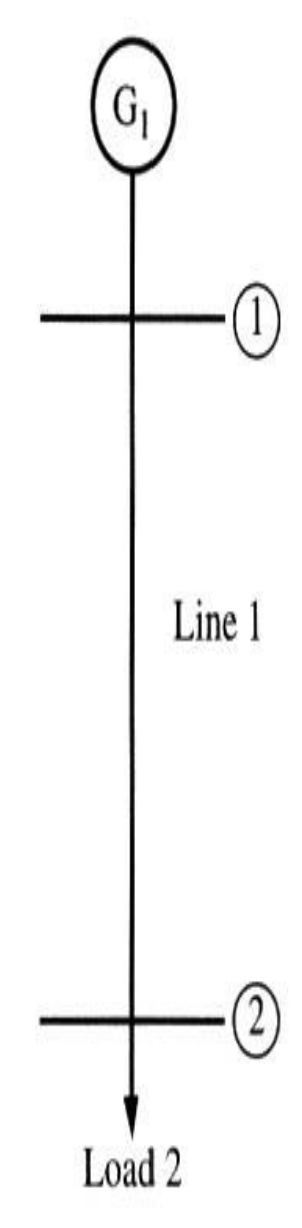
\includegraphics[height = 7cm]{img/figure51.png}
	\caption{Example 2 diagram.}
\end{figure}
\begin{enumerate}
	\item We start from calculating the bus admittance matrix $Y_{bus}$. The $Y_{ii}$ terms can be constructed by summing the admittances of all transmision lines connected to each bus, and the $Y_{ij}$ terms are the negative of the admittances of the line stretcing between busses $i$ and $j$. For instance, the term $Y_{11}$ is the sum of the admittances of all transmission lines connected to bus 1 (a single line in our case). The series admittance of line 1 is:
	\begin{gather}
		Y_{line1} = \frac{1}{Z_{line1}}= \frac{1}{0.1+j0.5} = 0.3846-j1.9231=Y_{11}
	\end{gather}
	Applying similar calculations to other terms, we complete the admittance matrix as:
	\begin{gather}
		Y_{bus} = \begin{bmatrix}
			0.3846-j1.9231 & -0.3846+j1.9231\\
			-0.3846+j1.9231 & 0.3846-j1.9231
		\end{bmatrix}
	\end{gather}
	\item Next, we select bus 1 as the slack bus since it is the only bus in the system connected to the generator. The voltage at bus 1 will be assumed $1.0\angle\SI{0}{\degree}$. 
	\item We select initial estimates for all bus voltages. Making a flat start, the initial voltage estimates at every bus are $1.0\angle\SI{0}{\degree}$. 
	\item Next, we write voltage equations for every other bus in the system. For bus 2:
	\begin{gather}
		V_2 = \frac{1}{Y_{22}}\left[ \frac{P_2-jQ_2}{V^*_{2,old}}-Y_{21}V_1 \right]
	\end{gather}
	Since the real and reactive powers \underline{suppled} at bus 2 are $P_2 = \SI{-0.3}{pu}$ and $Q_2 = \SI{0.2}{pu}$ and since $Y_s$ and $V_1$ are known, we may reduce the last equation:
	\begin{align}
		V_2 &= \frac{1}{0.3846 - j1.9231}\left[\frac{-0.3-j0.2}{V^*_{2,old}}-\left(\left(-0.3846+j1.9231\right)V_1\right)\right]\\
		&= \frac{1}{1.9612\angle\SI{-78.8}{\degree}}\left[\frac{0.3603\angle\SI{-146.3}{\degree}}{V^*_{2,old}}-\left(1.9612\angle\SI{101.3}{\degree}\right)\left(1\angle\SI{0}{\degree}\right)\right]
	\end{align}
	\item Next, we calculate an updated estimate of the voltages at each load bus in succession. In this problem we only need to calculate updated voltages for bus 2. since the voltage at the slack bus (bus 1) is assumed constant. We repeat this calculation until the voltage converges to a constant value. The initial estimate for the voltage is $V_{2,0} = 1\angle\SI{0}{\degree}$. The next estimate for the voltage is:
	\begin{align}
		V_{2,1} &= \frac{1}{1.9612\angle\SI{-78.8}{\degree}}\left[\frac{0.3603\angle\SI{-146.3}{\degree}}{V^*_{2,old}}-\left(1.9612\angle\SI{101.3}{\degree}\right)\left(1\angle\SI{0}{\degree}\right)\right]\\
		&= \frac{1}{1.9612\angle\SI{-78.8}{\degree}}\left[\frac{0.3603\angle\SI{-146.3}{\degree}}{1\angle\SI{0}{\degree}}-\left(1.9612\angle\SI{101.3}{\degree}\right)\left(1\angle\SI{0}{\degree}\right)\right]\\
		&= 1.0834\angle\SI{-9.0275}{\degree}
	\end{align}
	The new estimate for $V_2$ substituted back to the equation will produce the second estimate:
\end{enumerate}